\documentclass[11pt]{article}
\usepackage[a4paper,margin=1in]{geometry}
\usepackage{amsmath,amssymb}
\usepackage{graphicx}
\usepackage{booktabs}
\usepackage{xcolor}
\usepackage[colorlinks=true,linkcolor=blue,citecolor=blue,urlcolor=blue]{hyperref}
\usepackage{caption}
\captionsetup{font=small,labelfont=bf}

\graphicspath{{../reports/collaborator_2026-06/figures_solo/}}

\newcommand{\MKK}{M_{\mathrm{KK}}}
\newcommand{\epsK}{\varepsilon_K}
\newcommand{\TeV}{\,\mathrm{TeV}}

\title{\bf Is minimal (non-custodial) Randall--Sundrum still better than the
Standard Model on \emph{flavor}?\\[4pt]
\large A confirm-or-kill reassessment of the anarchic warped-flavor claim}
\author{5D-Neutrino-Mixing project --- quark-sector reassessment note}
\date{June 2026}

\begin{document}
\maketitle

\begin{abstract}
\noindent
We ask, narrowly and quantitatively, whether minimal anarchic Randall--Sundrum
(RS) makes \emph{any} flavor statement --- at an indirectly reachable
$\MKK$ --- that the Standard Model (SM) does not already make, and that is not
already collapsed to ``$\sim$\,SM.'' Working entirely from a $9.9\times10^{5}$-draw
anarchic forward ensemble (the literature ``strawman'' lane), with masses and
tree-level CKM \emph{fixed} and all flavor/CP/electroweak observables held out as
a test set, we build an \emph{SM-overlap scoreboard}: for every NP-sensitive
quark channel we compute the $\MKK$ below which a $>1\sigma$ deviation from the SM
is \emph{generic}, and overlay the scales the model must survive
($\epsK$ and the oblique $S,T,U$). The result is unambiguous. Every flavor
deviation has fallen below $1\sigma$ by $\MKK\!\approx\!1.9\TeV$, while survival
requires $\MKK\!\gtrsim\!19\TeV$ from $\epsK$ and $\gtrsim\!18\text{--}20\TeV$
irreducibly from oblique $T$ --- a full decade of separation. Custodial symmetry
relieves the electroweak floor ($\sim$16$\to$6\,TeV in our oblique proxy) but
leaves the $\epsK$ wall untouched, because $\epsK$ is a custodial-invariant
KK-gluon operator. We conclude (B): \emph{minimal anarchic RS retains exactly one
genuine virtue absent in the SM --- the geometric, single-input origin of both the
mass hierarchy and the RS-GIM FCNC-suppression pattern --- but as a predictive
flavor theory it no longer buys anything; every would-be prediction is
unobservable at any viable scale, and viability itself must be purchased with
custodial protection and explicit flavor alignment, structure the SM never
required.} Throughout, every floor is tagged with its model lane; the numbers
here are the \textbf{anarchic} (Lane A) floors by design.
\end{abstract}

\section{The question and a fair standard}
\label{sec:standard}

The interesting comparison is \emph{not} whether RS can fit the fermion masses and
the CKM matrix. In the bulk-fermion construction that is the premise: exponentially
different zero-mode overlaps, set by one $O(1)$ bulk-mass parameter $c$ per field,
turn anarchic $O(1)$ five-dimensional Yukawas into the observed 4D hierarchy. The
real question is whether, \emph{after} fitting masses and mixings, the same
geometry yields a distinctive, still-viable pattern of flavor and CP violation that
the SM does not already describe at least as well.

We therefore impose an explicit \textbf{fit-set / test-set split}. The fit set
contains only what RS is allowed to claim geometrically: quark masses and the
tree-level CKM angles and phase. The test set is everything else --- neutral-meson
mixing ($\epsK,\Delta m_K,\Delta m_{B_{d,s}}$, the $B$ mixing phases), $D^0$
mixing, and electroweak precision ($S,T,U$, $Z\to b\bar b$). This is also what
makes the comparison fair to the SM: the SM benchmark uses tree-level CKM inputs
only, so no possible new physics in the mixing observables is fed back into the
reference fit used to test those same observables. ``RS does better'' then means a
\emph{predictive surplus} on the test set after the fit set is fixed --- not merely
extra flexibility.

Two benchmarking points must be stated up front. First, the anarchic
$\epsK$ wall (Sec.~\ref{sec:epsK}) is the baseline the literature
\emph{criticizes}; it is not ``our'' production model. Second, RS does
\textbf{not} reduce the number of physical flavor parameters relative to the SM:
the quark sector still carries two complex $5$D Yukawa matrices plus bulk-mass
matrices~\cite{APS}. The claim was always \emph{structure from anarchy plus
localization}, never fewer knobs. RS must therefore win, if at all, on structure,
prior-naturalness, and out-of-sample predictions.

\paragraph{Space of honest conclusions.}
We pre-registered three outcomes: (A) RS wins narrowly --- some generic anarchic
correlation, distinct from the SM at $>1\sigma$ of current resolution, realized at
an $\MKK$ that simultaneously survives $\epsK$ \emph{and} $S,T,U$; (B) RS is reduced
to a mass-hierarchy mechanism plus a non-falsifiable FCNC correlation; (C) RS
flavor adds nothing whatever. We commit to landing wherever the data point, by
\emph{trying to rescue (A) and documenting the failure}. We explicitly decline
(C): the geometric-hierarchy virtue is real and a referee would correctly defend
it. The spine of the paper is one question: \emph{is there any $\MKK$ at which a
generic anarchic point both survives and still shows a measurable deviation?}

\section{What RS genuinely buys --- and what it does not}
\label{sec:virtue}

The one SM-absent virtue is worth steelmanning. The same wavefunction overlap
$f(c)$ that produces the five-decade mass hierarchy also sets the flavor-changing
KK couplings, with the celebrated RS-GIM scaling
\begin{equation}
  (\delta_{\rm FCNC})_{ij}\ \sim\ \frac{\sqrt{m_i m_j}}{v}\,,
\end{equation}
so that light-fermion FCNCs are automatically suppressed by the \emph{same} input
that makes those fermions light. A single geometric structure generates two
phenomena the SM merely parametrizes (the hierarchy) or assumes (GIM). That is a
genuine explanatory economy, and it is the strongest thing RS has to say about
flavor.

What RS does \emph{not} buy is equally important and is the SM's side of the
ledger. The SM already accounts for \emph{all} observed flavor and CP violation as
a precision null test: once masses and tree-level CKM are fixed, the loop-level
mixing observables are reproduced with \emph{no added structure}, no new
parameters, and no tuning. RS, to remain viable, must add custodial protection (for
$T$, Sec.~\ref{sec:cures}) and explicit flavor alignment (for $\epsK$), and even
then does not reduce the parameter count. So the contest is asymmetric in a way the
rest of this note quantifies: RS offers a \emph{story} the SM lacks, but on
\emph{predictions} the SM is at least as good and structurally cheaper.

\section{The recentered electroweak landscape (2008\,$\to$\,2025)}
\label{sec:recenter}

A reassessment is timely now, and was not in 2008, for three reasons. The Higgs has
been found, moving RS's \emph{raison d'\^etre} from ``trigger EWSB'' to ``flavor +
composite Higgs'' and re-introducing the little hierarchy $v/f$. The $\epsK$ SM
tension sharpened with 2025 lattice inputs. And --- the cleanest lever --- the
oblique ellipse \textbf{recentered on the SM}. Figure~\ref{fig:st} overlays the
2008 fit (CGHNP, $S=0.07\pm0.10$, $T=0.16\pm0.10$) against PDG-2025
($S=0.026\pm0.075$, $T=0.047\pm0.066$, $\rho=0.90$; and the $U$-free variant). The
2008 ellipse sat at \emph{positive} $T$, exactly where a minimal RS KK tower wants
to live; the 2025 ellipse sits on the SM point, so the same RS $T$-wedge is now
disfavored.

\begin{figure}[t]
  \centering
  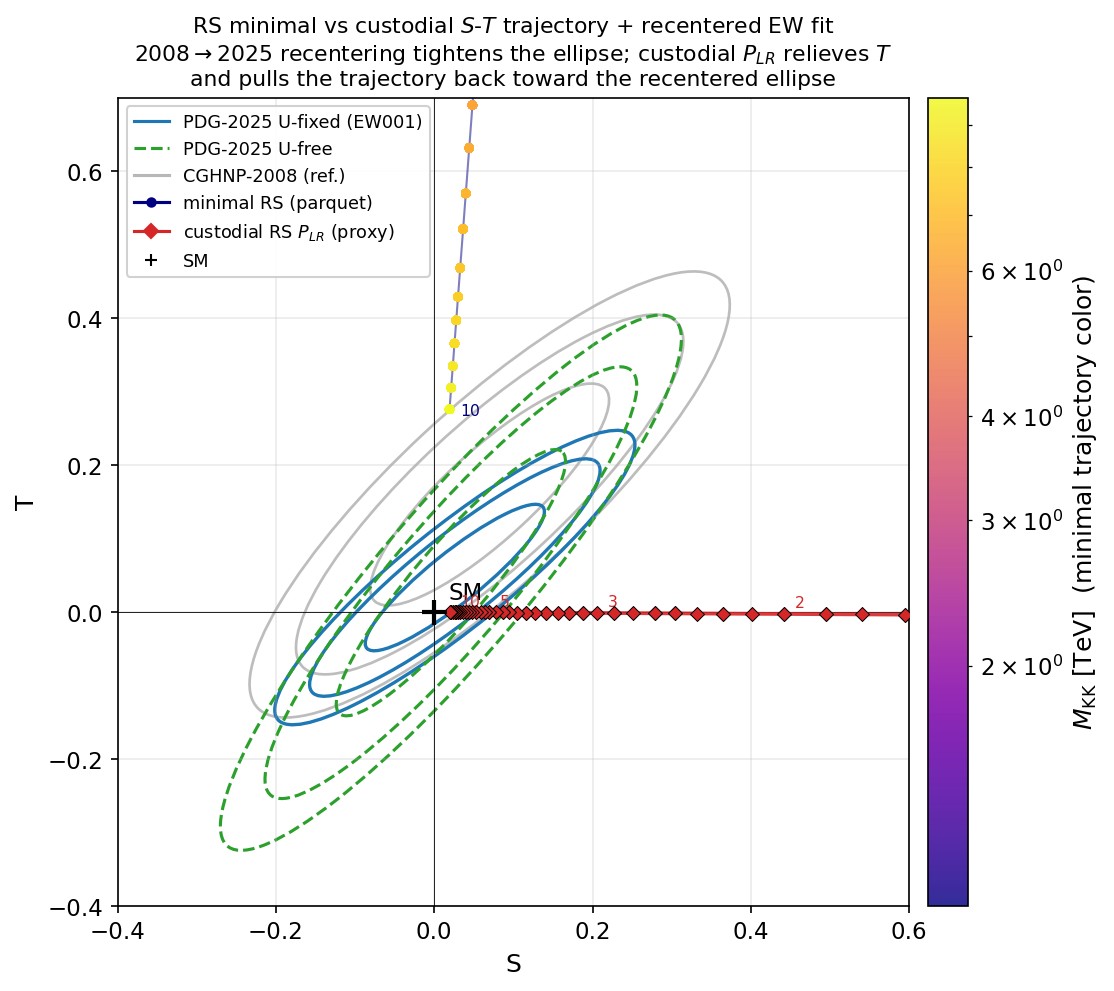
\includegraphics[width=0.78\textwidth]{solo_ST_recentered.png}
  \caption{Recentered $S$--$T$ plane. The minimal RS proxy (navy, colored by
  $\MKK$) climbs steeply in $T$, leaving every ellipse; the custodial $P_{LR}$
  proxy (red) hugs $T\approx0$ along the $S$ axis. The 2008$\to$2025 recentering
  (grey$\to$blue/green ellipses) tightens the fit \emph{and} moves it onto the SM,
  raising the minimal oblique floor (Table~\ref{tab:oblique}).}
  \label{fig:st}
\end{figure}

Quantitatively, the recentering \emph{raises} the minimal floor and custodial
\emph{lowers} it (Table~\ref{tab:oblique}). Against PDG-2025 (U-fixed) the minimal
oblique proxy is excluded up to $16.0\TeV$, versus $10.4\TeV$ against the looser
2008 ellipse --- the tighter, recentered fit is a real lever. Custodial $P_{LR}$
protection drops the same floor to $5.8\TeV$ (the residual is set by $S$, which
custodial does not protect). These are oblique-only proxy floors at fixed
$(v,\sin^2\theta_W,L{=}35)$; the lane-independent $S,T,U$ \emph{existence} floor
from the full scan is $18\text{--}20\TeV$ (Sec.~\ref{sec:STU}).

\begin{table}[t]
  \centering
  \caption{C1 oblique floors: largest $\MKK$ [TeV] excluded at $95\%$ by the $S,T$
  proxy, for each EW fit. Recentering raises the minimal floor; custodial relieves
  it at every fit but cannot reach the few-TeV regime because $S$ is unprotected.}
  \label{tab:oblique}
  \begin{tabular}{lccc}
    \toprule
    EW model & CGHNP-2008 & PDG-2025 ($U$-fixed) & PDG-2025 ($U$-free) \\
    \midrule
    minimal RS        & 10.4 & \textbf{16.0} & 13.2 \\
    custodial $P_{LR}$ & \phantom{0}7.6 & \phantom{0}\textbf{5.8} & \phantom{0}4.6 \\
    \bottomrule
  \end{tabular}
\end{table}

\section{The flavor wall: anarchy over-saturates $\epsK$}
\label{sec:epsK}

The strongest generic bound on anarchic RS comes from the kaon system, where the
left--right $\Delta S=2$ operator $C_4$ is chirally and RG-enhanced.
Figure~\ref{fig:epsK} shows the anarchic $|\epsK|$ cloud with $5/50/95\%$
quantiles. The $95\%$ quantile crosses the experimental window only near
$\MKK\!\sim\!10\TeV$ (paper-era inputs); with current inputs the \emph{median}
floor is higher. Figure~\ref{fig:zbb} (right) makes the mechanism explicit: the KK
contribution to the kaon $M_{12}$ is $\sim\!10^2\times$ more important in its
imaginary (CP-violating) part than its real part, the hallmark of the
$C_4$-dominated $\epsK$ problem.

\begin{figure}[t]
  \centering
  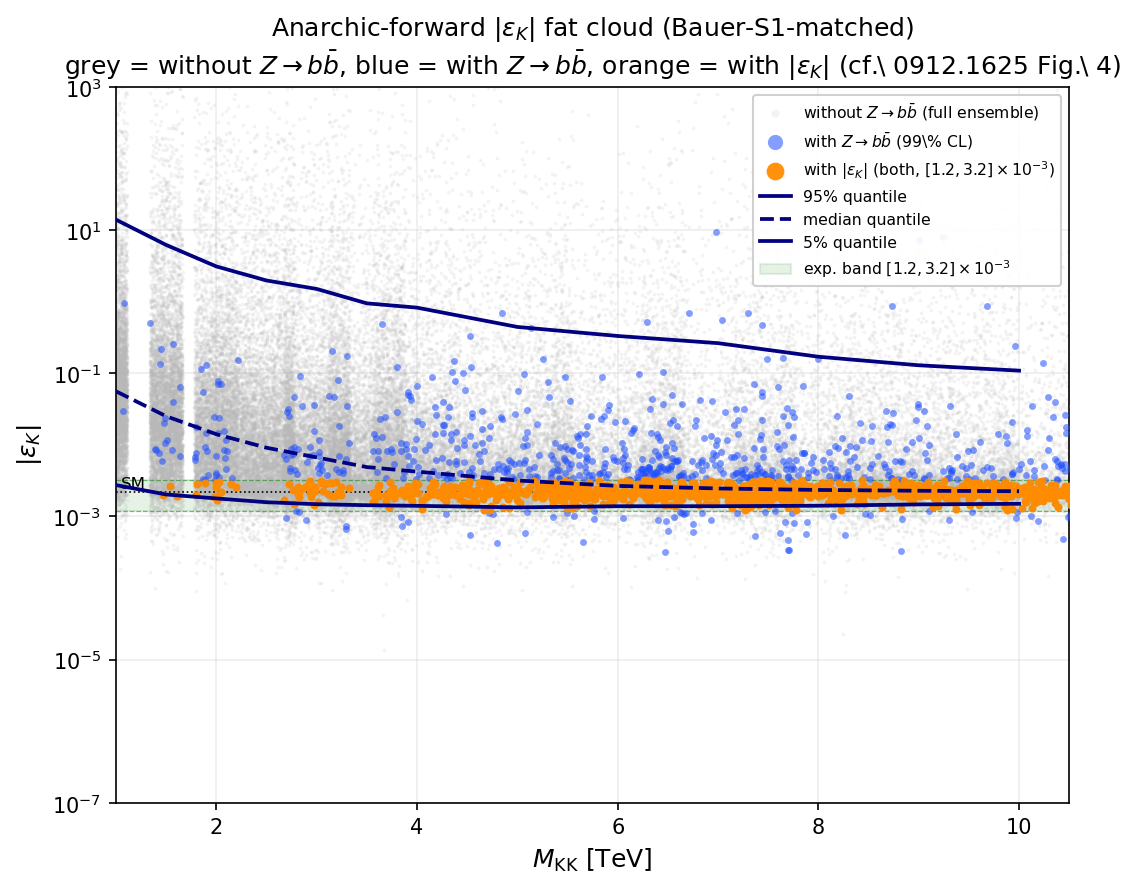
\includegraphics[width=0.70\textwidth]{solo_epsK_cloud.png}
  \caption{Anarchic (Lane A) $|\epsK|$ cloud vs $\MKK$: grey $=$ mass+CKM
  consistent (no $Z\to b\bar b$ cut), blue $=$ also $Z\to b\bar b$ consistent,
  orange $=$ also in the $\epsK$ window. The $95\%$ quantile reaches the window edge
  near $10\TeV$ (paper-era); the typical wall is higher with current inputs.}
  \label{fig:epsK}
\end{figure}

The wall is robust to the dominant systematic, $|V_{cb}|$, which controls $\epsK^{\rm
SM}$ and hence the NP budget. Rescaling the per-draw $\epsK$ exactly across the
$|V_{cb}|$ range gives an anarchic median floor of
\[
  \epsK\ \text{floor}\ \approx\ 9\text{--}24\TeV
\]
(inclusive vs.\ exclusive $|V_{cb}|$, realized-Im vs.\ modulus phase convention).
Every value is an order of magnitude above the flavor-\emph{deviation} floor of
Sec.~\ref{sec:scoreboard}, so the verdict does not depend on this choice; the much-
quoted $5\sigma$ $\epsK$ tension is corroborating, not load-bearing.

\section{The irreducible wall: oblique $T$ and the existence floor}
\label{sec:STU}

Unlike flavor, which can in principle be tuned or aligned away, the oblique $T$
parameter has \emph{no} Yukawa freedom: it is generated by the KK tower's
electroweak mixing and is essentially the same for every anarchic draw.
Figure~\ref{fig:exist} separates the \emph{existence} floor (best/tuned point,
per-$\MKK$ minimum) from the \emph{typical} floor (median). For the flavor
observables the existence floor crashes below $1\TeV$ --- a tuned point can always
evade any single flavor constraint --- but the \emph{combined} existence floor sits
at $18\text{--}20\TeV$, set by $S,T,U$, which the minimum tracks the median because
there is nothing to tune. This is the lane-independent wall: it stands in every
flavor scenario, anarchic or aligned.

\begin{figure}[t]
  \centering
  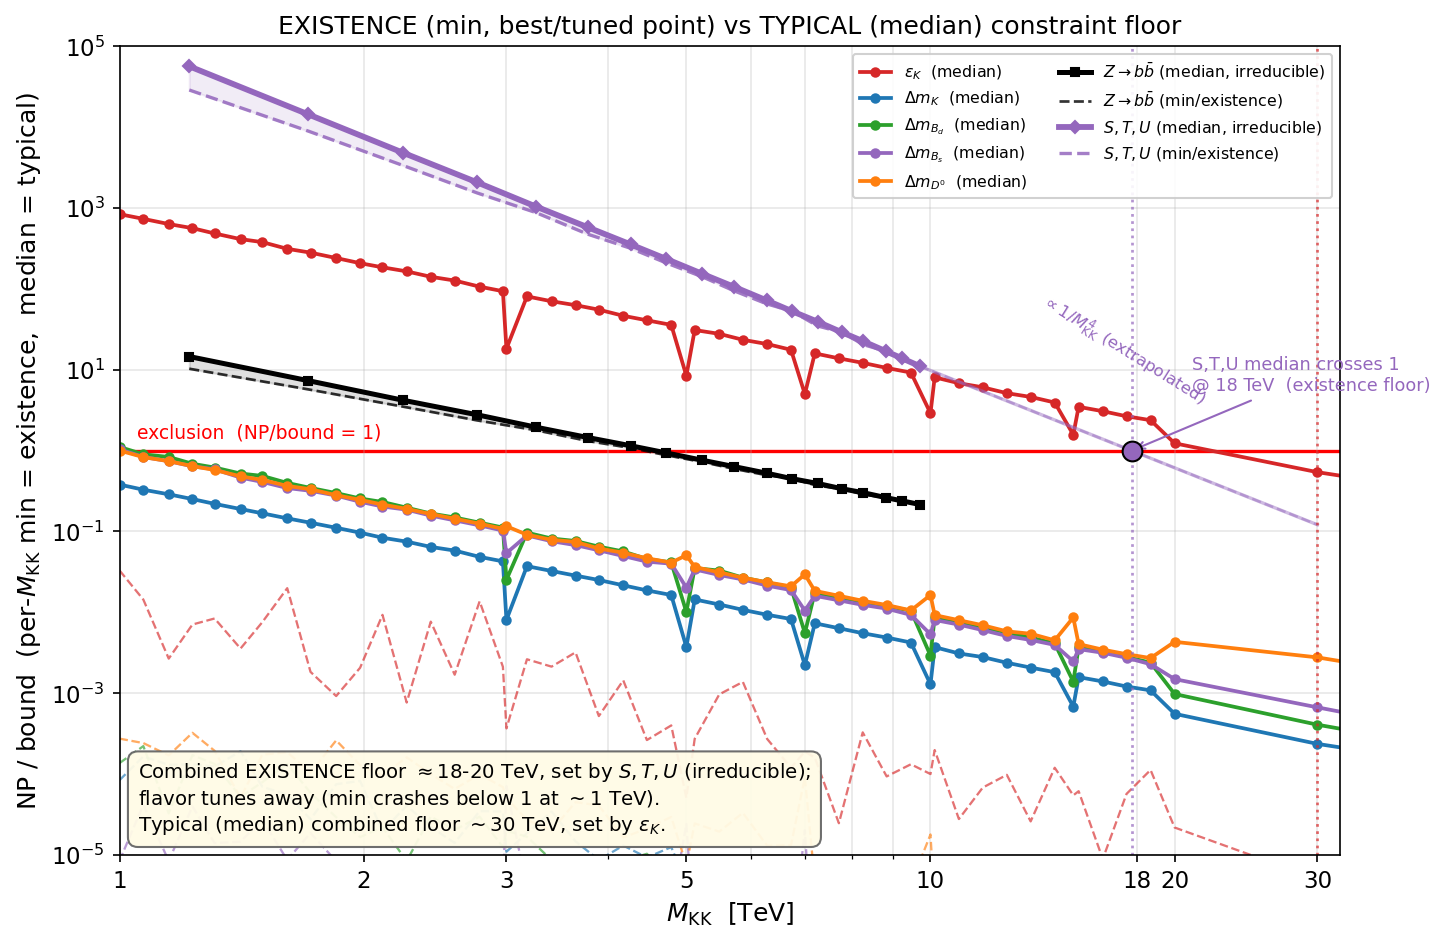
\includegraphics[width=0.86\textwidth]{solo_existence_vs_typical.png}
  \caption{Existence (min, best point) vs typical (median) floors. Flavor tunes
  away (its min crashes below $1\TeV$); $S,T,U$ does not (min $\approx$ median),
  setting an irreducible existence floor of $18\text{--}20\TeV$. The typical
  combined floor ($\sim$30\,TeV here) is set by $\epsK$.}
  \label{fig:exist}
\end{figure}

\section{The decisive test: the SM-overlap scoreboard}
\label{sec:scoreboard}

We now run the (A)-vs-(B) discriminator directly. From the co-registered
$9.9\times10^5$-draw ensemble of complex NP $M_{12}$ values for $K/B_d/B_s/D$ (gated
to the $1.1\times10^5$ mass+CKM-consistent draws), we compute, per channel and per
$\MKK$ tile, the generic (median) deviation from the SM in units of the current
experimental resolution. Crucially, the $B$-meson \emph{phases} are computed
KI-correctly, from the stored complex $M_{12}$ against a \emph{complex} SM box,
\begin{equation}
  \phi_q^{\Delta} \;=\; \arg\!\big(1 + M_{12}^{\rm NP}/M_{12}^{\rm SM\text{-}box}\big),
  \qquad
  M_{12}^{\rm SM\text{-}box}\ \text{complex},
\end{equation}
not a real-$M_{12}^{\rm SM}$ adapter (which is not rephasing-invariant). The
channels and their $1\sigma$ sensitivities are $\phi_s$ ($16$\,mrad), $C_{B_s}$
($0.09$), $\sin2\beta$ ($0.017$), $C_{B_d}$ ($0.08$), and $D^0$ amplitude (vs.\
$\Delta m_D^{\rm exp}$, long-distance-dominated and hence a conservative bound, not
a hard exclusion).

\begin{figure}[t]
  \centering
  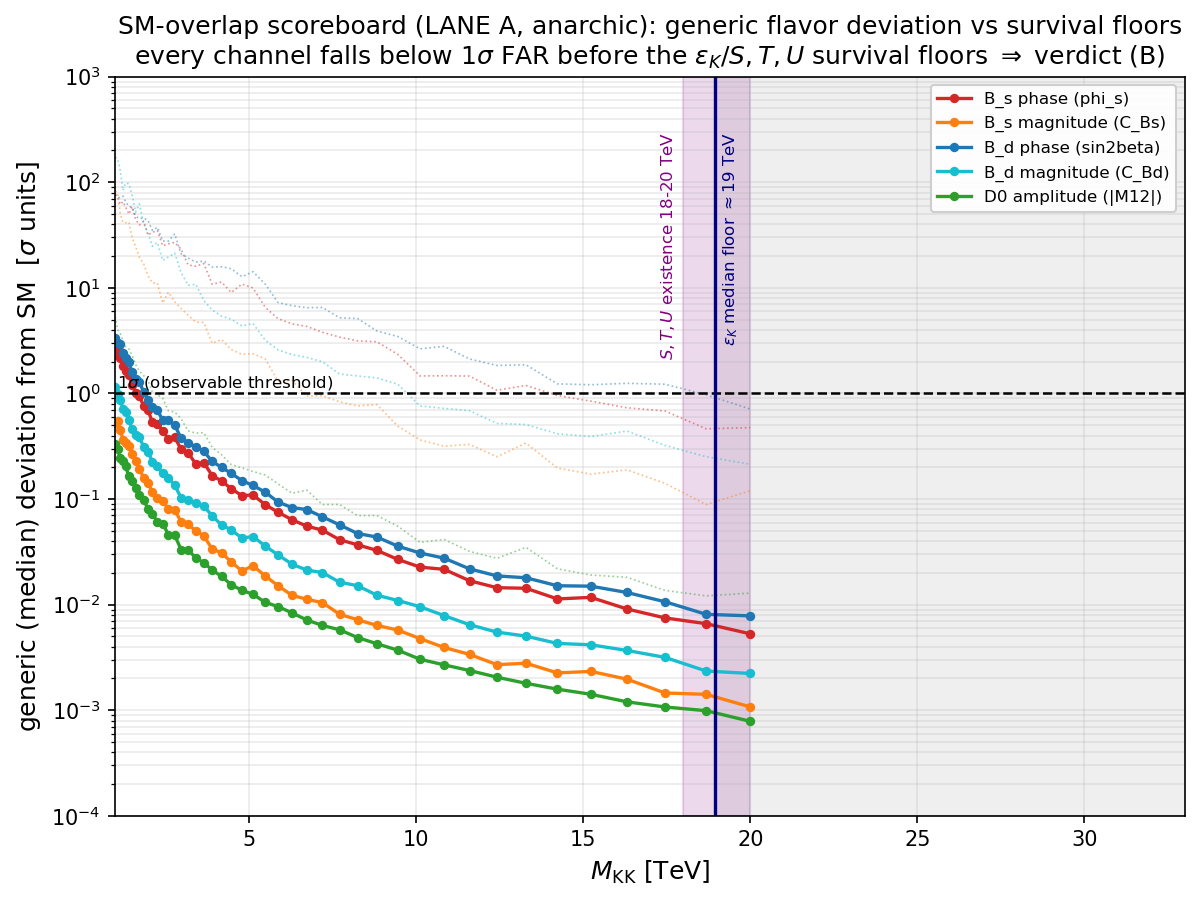
\includegraphics[width=0.86\textwidth]{solo_sm_overlap_scoreboard.png}
  \caption{\textbf{The decisive figure.} Generic (median) deviation from the SM, in
  $\sigma$ units, vs $\MKK$, for every NP-sensitive quark channel (dotted $=95\%$
  tail). The dashed line is the $1\sigma$ observability threshold; the shaded bands
  are the $\epsK$ median and $S,T,U$ existence survival floors. Every channel falls
  below $1\sigma$ by $\MKK\!\approx\!1.9\TeV$ --- a full decade below the survival
  floors. At the survival floor all channels sit at $10^{-2}\text{--}10^{-3}\sigma$.}
  \label{fig:scoreboard}
\end{figure}

The result (Fig.~\ref{fig:scoreboard}, Table~\ref{tab:scoreboard}) is decisive. The
most NP-sensitive channel, the $B_d$ mixing phase, has a generic deviation that
crosses below $1\sigma$ at $\MKK=1.9\TeV$; the others cross even lower, and $C_{B_s}$
and $D^0$ never reach $1\sigma$ even at $1\TeV$. Meanwhile survival requires
$\MKK\gtrsim19\TeV$ ($\epsK$) and $\gtrsim18\text{--}20\TeV$ ($S,T,U$). At the
survival floor every channel sits at $10^{-2}\text{--}10^{-3}\sigma$ --- utterly
SM-like. The robustness is double: even the $95\%$ tail (the most NP-active draws)
is sub-$1\sigma$ for $\MKK\ge18.95\TeV$ (the $B_d$ phase tail crosses $1\sigma$ at
$18.5\TeV$, just inside the $S,T,U$ band, and is $0.71\sigma$ by $20\TeV$). There is
no $\MKK$ at which a surviving anarchic point shows an observable flavor deviation.
\textbf{Conclusion (A) is dead; (B) is confirmed.}

\begin{table}[t]
  \centering
  \caption{SM-overlap scoreboard: $\MKK$ [TeV] below which a $>1\sigma$ deviation is
  \emph{generic} (median draw), per channel, vs the survival floors. The largest
  deviation floor ($1.9\TeV$) is a decade below the binding survival floor.}
  \label{tab:scoreboard}
  \begin{tabular}{lc}
    \toprule
    Channel (quark) & generic $>1\sigma$ deviation floor [TeV] \\
    \midrule
    $B_d$ phase ($\sin2\beta$) & 1.87 \\
    $B_s$ phase ($\phi_s$)     & 1.64 \\
    $B_d$ magnitude ($C_{B_d}$) & 1.06 \\
    $B_s$ magnitude ($C_{B_s}$) & never reaches $1\sigma$ \\
    $D^0$ amplitude            & never reaches $1\sigma$ \\
    \midrule
    \emph{survival}: $\epsK$ median & $\sim$19 (band 9--24) \\
    \emph{survival}: $S,T,U$ existence & 18--20 \\
    \bottomrule
  \end{tabular}
\end{table}

\section{Electroweak side notes}
\label{sec:ew}

Two corrections keep the diagnosis honest. First, $Z\to b\bar b$ is \emph{not} the
driver: a corrected treatment puts its floor near $5\TeV$ (Fig.~\ref{fig:zbb}), well
below $\epsK$ and $S,T,U$, so the binding constraints are genuinely $\epsK$ and
$T$, not $Z\to b\bar b$. Second, the kaon $\mathrm{Im}/\mathrm{Re}$ asymmetry of
Fig.~\ref{fig:zbb} (right, $\sim10^2$) is the fingerprint of the $C_4$ operator and
confirms our matching against the published anarchic results.

\begin{figure}[t]
  \centering
  \begin{minipage}{0.49\textwidth}\centering
    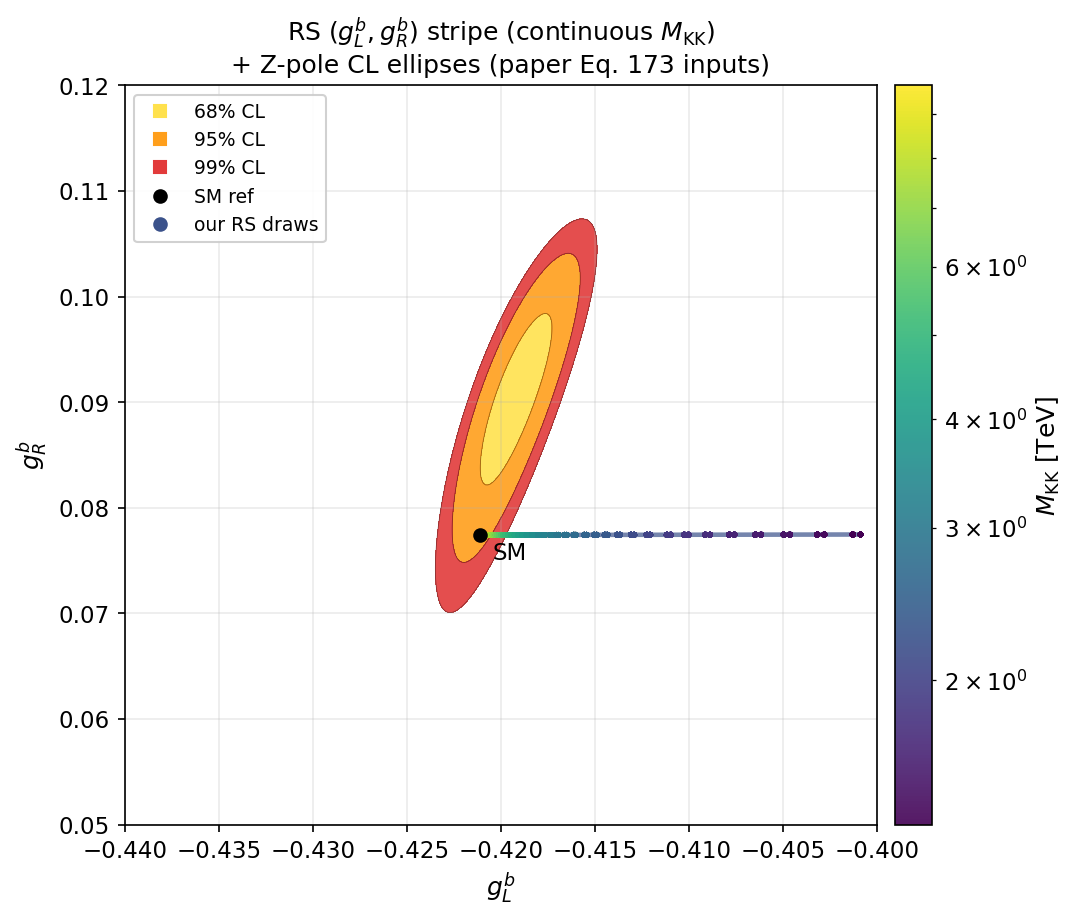
\includegraphics[width=\textwidth]{solo_Zbb_gLgR.png}
  \end{minipage}\hfill
  \begin{minipage}{0.49\textwidth}\centering
    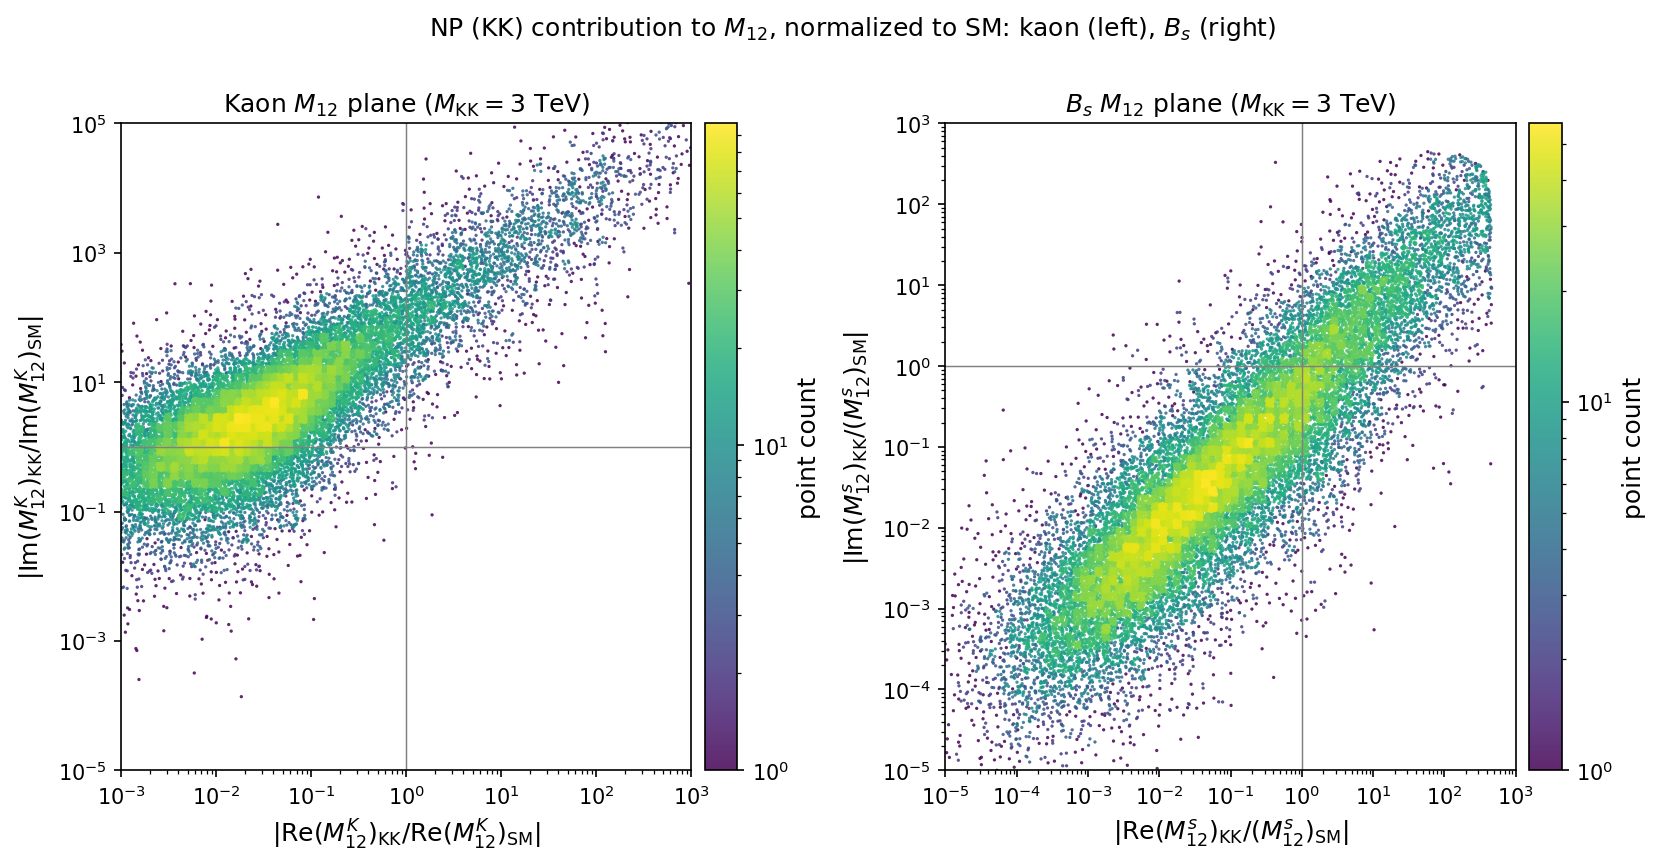
\includegraphics[width=\textwidth]{solo_ReIm_M12.png}
  \end{minipage}
  \caption{Left: $(g_L^b,g_R^b)$ stripe with the $Z$-pole CL ellipses --- the
  $Z\to b\bar b$ floor is $\sim$5\,TeV, not a driver. Right: the kaon (and $B_s$)
  $M_{12}$ planes, showing the $\sim$$10^2$ imaginary-over-real KK enhancement that
  drives $\epsK$.}
  \label{fig:zbb}
\end{figure}

\section{The cures and what they cost}
\label{sec:cures}

What would it take to rescue a low $\MKK$? Two distinct additions, neither for free.

\paragraph{Custodial protection fixes the electroweak sector, not $\epsK$.}
The custodial $SU(2)_L\!\times\!SU(2)_R\!\times\!U(1)_X\!\times\!P_{LR}$ structure
cancels the leading $T$ (SU(2)$_R$~\cite{ADMS}) and protects the $Z\,b_L\bar b_L$
vertex (the discrete $P_{LR}$~\cite{ACDP}), relieving the oblique floor from
$\sim$16\,TeV to $\sim$6\,TeV (Table~\ref{tab:oblique}); the residual is set by $S$,
which custodial does \emph{not} protect. But $\epsK$ is a color-octet KK-gluon
left--right ($C_4$) operator, a \emph{singlet} under the electroweak custodial group,
and is therefore untouched by custodialization. This is not an inference from operator
counting alone: Blanke \emph{et al.}~\cite{Blanke} computed the full $\Delta F=2$ set
\emph{inside the custodial model} and still find $\MKK\gtrsim18\TeV$ (fine-tuning
$<20$) / $\gtrsim30\TeV$ ($<10$); Cs\'aki--Falkowski--Weiler~\cite{CFW} make the split
explicit --- custodial passes electroweak precision at $\sim$3\,TeV while $\epsK$
forces $\MKK\gtrsim21\text{--}33\TeV$. Figure~\ref{fig:ladder} collects this: the
electroweak floors ($S,T,U$ and $Z\to b\bar b$) move to a few TeV under custodial,
while the $\epsK$ wall does not move at all, in our numbers and in the literature
alike. Custodial buys electroweak viability, and nothing on flavor.

\begin{figure}[t]
  \centering
  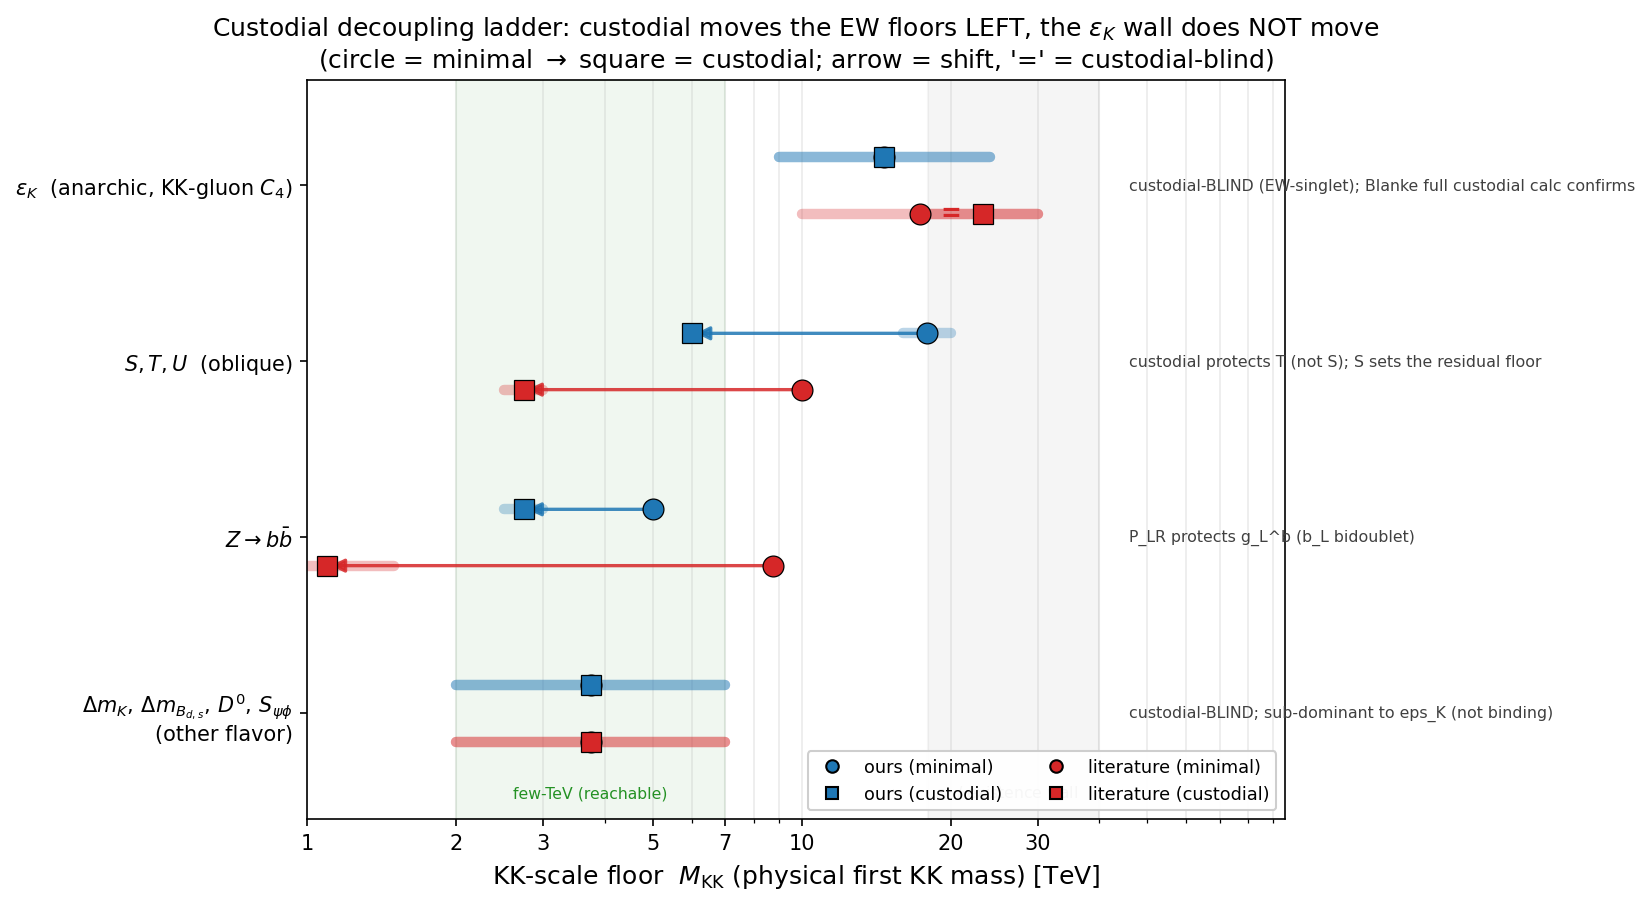
\includegraphics[width=0.92\textwidth]{custodial_decoupling_ladder.png}
  \caption{\textbf{Custodial decoupling ladder.} Per-constraint KK-scale floor,
  minimal (circle) $\to$ custodial (square), ours (blue) vs literature (red). The
  electroweak constraints ($S,T,U$, $Z\to b\bar b$) shift \emph{left} under
  custodialization (arrows); $\epsK$ and the other flavor constraints do not move
  (``$=$''), because the binding kaon operator is a color-octet KK-gluon, blind to
  the electroweak custodial group. Literature anchors: \cite{ADMS,CPSW,CFW,Blanke,Bauer}.
  (Leading custodial physics only; the subleading custodial flavor effects ---
  EW KK-boson $\Delta F=2$, custodian loops --- are not in our proxy and do not change
  the $\epsK$ wall.)}
  \label{fig:ladder}
\end{figure}

\paragraph{Flavor alignment fixes $\epsK$, by adding structure.}
Aligning or degenerating the flavor sector --- 5D MFV, a horizontal $U(1)$, or a
$U(3)$ degeneracy of the right-handed down quarks (Bauer's ``S2'') --- can drive the
$\epsK$ floor from $\sim$19\,TeV (anarchic, S1) down toward $\sim$1.8\,TeV
(Fig.~\ref{fig:s2}). But this trades ``anarchy \emph{predicts}'' for ``symmetry
\emph{imposes}'': the cloud stays anarchically fat, it simply gains far more
$\epsK$-consistent points once the right-handed down mixing that feeds $C_4$ is
removed by hand. A down-aligned cure must additionally pay the $D^0$/charm
cross-check, since relieving the kaon can shift residual flavor violation into the
up sector ($D^0$ is conservative here, being long-distance-dominated). The net
flavor structure is then no more predictive, and no more economical, than the SM's.

\begin{figure}[t]
  \centering
  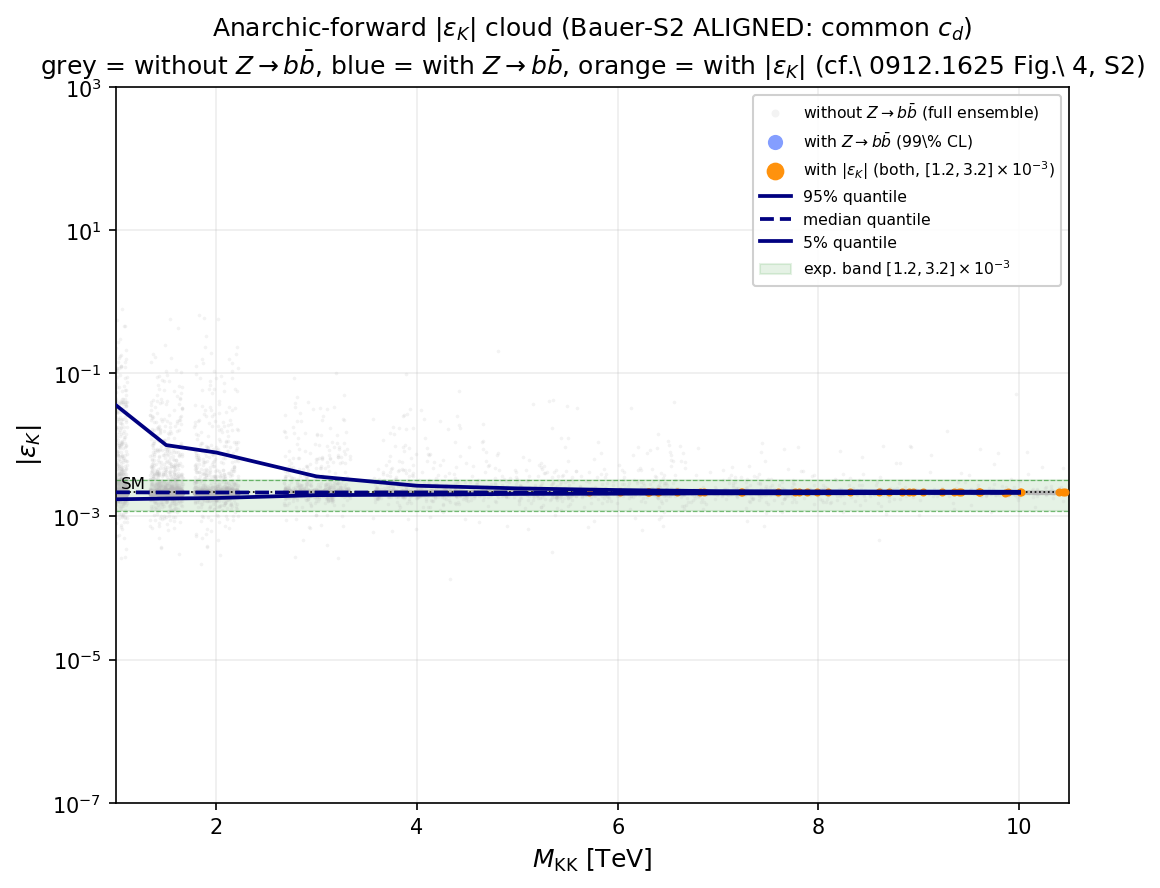
\includegraphics[width=0.62\textwidth]{solo_epsK_cloud_S2.png}
  \caption{Alignment endpoint (Bauer-S2, common right-handed down $c_d$ via a
  $U(3)$ degeneracy): the cloud stays fat but gains $\epsK$-consistent points,
  dropping the floor toward $\sim$1.8\,TeV --- a cure that imposes structure rather
  than predicting it.}
  \label{fig:s2}
\end{figure}

\section{Verdict}
\label{sec:verdict}

We land on (B). Minimal anarchic RS retains exactly one virtue the SM lacks: a
single geometric input generates both the fermion-mass hierarchy and the RS-GIM
FCNC-suppression pattern. That virtue is real, and we do not dispute it. But as a
\emph{flavor theory} it no longer buys a viable TeV-scale prediction. Run forward
with anarchy, the same input forces $\MKK\gtrsim9\text{--}24\TeV$ from $\epsK$ and
$\gtrsim18\text{--}20\TeV$ irreducibly from oblique $T$, while \emph{every} would-be
flavor prediction --- $\phi_s$, $S_{\psi\phi}$, $C_{B_d}$, $C_{B_s}$, the $D^0$
phase --- has collapsed onto the SM point by $\sim$2\,TeV, a decade below the
survival floor. The recentering of the $S$--$T$ ellipse onto the SM disfavors the
RS $T$-wedge that 2008 data tolerated; custodial symmetry rescues the electroweak
sector but not $\epsK$; and alignment rescues $\epsK$ only by importing the flavor
structure that anarchic RS was supposed to make unnecessary.

The honest bottom line is symmetric. \textbf{What RS does that the SM does not:} it
tells a geometric story for why the hierarchy and GIM look the way they do.
\textbf{What the SM does better:} it accounts for all observed flavor and CP
violation as a loop-level null test, with no added structure, no parameter
reduction conceded by RS, and none of the custodial-plus-alignment scaffolding RS
needs merely to survive. The RS-GIM correlation is real but non-falsifiable at any
reachable scale; on the predictions that could distinguish the two theories, the SM
is at least as good and structurally cheaper. Minimal warped flavor today is a
mechanism for the mass hierarchy --- no longer a competitive theory of flavor.

\paragraph{Lane discipline.} All floors quoted here are the \textbf{anarchic}
(Lane~A) floors --- the literature strawman the note interrogates --- not the
project's simplified-MFV production lane ($\sim$7\,TeV, no $V_{\rm 5KM}$) or the
fully aligned FPR ideal ($\sim$2\,TeV). The 7$\to$2\,TeV gap in the production
program is exactly the principled alignment (Sec.~\ref{sec:cures}) not yet wired in;
it does not affect the anarchic verdict above.

\begin{thebibliography}{9}
\small
\bibitem{APS} K.~Agashe, G.~Perez, A.~Soni, \emph{Flavor structure of warped extra
dimension models}, Phys.\ Rev.\ D \textbf{71} (2005) 016002 [hep-ph/0408134].
\bibitem{CGHNP} S.~Casagrande, F.~Goertz, U.~Haisch, M.~Neubert, T.~Pfoh,
\emph{Flavor Physics in the Randall-Sundrum Model: I}, JHEP \textbf{10} (2008) 094
[arXiv:0807.4937] (minimal-RS $S,T,U$ and $Z\to b\bar b$; the custodial $\Delta T$
distillation, Eq.~153).
\bibitem{Bauer} M.~Bauer, S.~Casagrande, U.~Haisch, M.~Neubert, \emph{Flavor Physics
in the Randall-Sundrum Model: II}, JHEP \textbf{09} (2010) 017 [arXiv:0912.1625].
\bibitem{Blanke} M.~Blanke, A.~J.~Buras, B.~Duling, S.~Gori, A.~Weiler,
\emph{$\Delta F=2$ Observables and Fine-Tuning in a Warped Extra Dimension with
Custodial Protection}, JHEP \textbf{03} (2009) 001 [arXiv:0809.1073].
\bibitem{ADMS} K.~Agashe, A.~Delgado, M.~J.~May, R.~Sundrum, \emph{RS1, Custodial
Isospin and Precision Tests}, JHEP \textbf{08} (2003) 050 [hep-ph/0308036].
\bibitem{ACDP} K.~Agashe, R.~Contino, L.~Da Rold, A.~Pomarol, \emph{A custodial
symmetry for $Z b\bar b$}, Phys.\ Lett.\ B \textbf{641} (2006) 62 [hep-ph/0605341].
\bibitem{CPSW} M.~Carena, E.~Pont\'on, J.~Santiago, C.~E.~M.~Wagner, \emph{Light
Kaluza-Klein states in Randall-Sundrum models with custodial $SU(2)$} and
\emph{Electroweak constraints on warped models with custodial symmetry},
Nucl.\ Phys.\ B \textbf{759} (2006) 202 / \textbf{767} (2007) 54 [hep-ph/0607106,
hep-ph/0701055].
\bibitem{CFW} C.~Cs\'aki, A.~Falkowski, A.~Weiler, \emph{The Flavor of the Composite
Pseudo-Goldstone Higgs}, JHEP \textbf{09} (2008) 008 [arXiv:0804.1954].
\bibitem{FPR} A.~L.~Fitzpatrick, G.~Perez, L.~Randall, \emph{A GIM mechanism from
extra dimensions}, [arXiv:0710.1869].
\bibitem{PDG2025} Particle Data Group, electroweak review (oblique $S,T,U$ fit,
2025; Table~10.8, $U$-fixed and $U$-free).
\bibitem{FLAG} FLAG Review 2024, lattice averages for kaon and $B$-meson mixing
matrix elements.
\end{thebibliography}

\end{document}
